\documentclass[class=book, crop=false]{standalone}
\usepackage[subpreambles=true]{standalone}
\usepackage{/home/mark/Documents/gradschool/research/thesis/preamble}
\usepackage{import}

\begin{document}

\chapter{Exceptional Cases}
\label{exceptional}
In the previous chapter we were able to show that $U_+$ is not finitely generated for a large family of Coxeter groups $W$ with labels $a\le b\le c.$ These results were based on assuming $b\ge 4$ which allowed us to show that $\D$ was infinite and proceed from there. In fact, we didn't even describe all of the chambers in $\D,$ just an infinite family. However, the same approach will not work in the remaining cases because of the following lemma.
\begin{lemma} If $W$ is a Coxeter group with labels $a\le b\le c$ as before, then $\D=\alpha_1\cap \alpha_n\cap \beta\cap \beta'$ as defined in the previous chapter is infinite if and only if $b\ge 4.$
	\label{lem:infD}
\end{lemma}
\begin{proof}
	We know by Lemma \ref{lem:infmany} that $\D$ is infinite if $b\ge 4.$ Thus it remains to show that $\D$ is finite if $b=3.$ If $b=3$ then $a=3$ also, and by definition of $a,b,c$ this means $m(s,t)=m(s,u)=3.$ We will also recall the definition of $\D=\alpha_1\cap \alpha_n\cap \beta \cap \beta'$ where
	\begin{align*}
	\alpha_1&=\{D\in \Sigma|d(D,C)<d(D,tC)\}=\{w\in W|\ell(w)<\ell(tw)\}\\
	\alpha_n&=\{D\in \Sigma|d(D,C)<d(D,uC)\}=\{w\in W|\ell(w)<\ell(uw)\}\\
	\beta&=\{D\in \Sigma|d(D,tC)<d(D,tsC)\}=\{w\in W|\ell(tw)<\ell(stw)\}\\
	\beta'&=\{D\in \Sigma|d(D,uC)<d(D,usC)\}=\{w\in W|\ell(uw)<\ell(suw)\}
\end{align*}

Let $w\in W$ and suppose $\ell(w)\ge 2.$ Then we can write $w=s_1s_2w'$ where $\ell(w')=\ell(w)-2.$ If $s_1=t$ then we have
\[
	\ell(tw)=\ell(s_2w')=\ell(w)-1<\ell(w)
\]
which shows $w\not\in \alpha_1$ and thus $w\not\in \D.$ A similar argument shows that $w\not\in \D$ if $s_1=u.$

Now we assume $s_1=s$ and so we can also assume $s_2=t,u.$ First let $s_2=t$ so that $w=stw'.$ If $w\not\in \alpha_1$ then $w\not\in \D$ and so we will suppose $w\in\alpha_1.$ Now we can see
\[
	\ell(stw)=\ell(ststw')=\ell(sstsw')=\ell(tsw')\le \ell(w')+2=\ell(w)<\ell(tw)
\]
and thus $w\not\in \D.$ A similar argument shows that $w\not\in \D$ if $s_2=u.$

We have shown that if $\ell(w)\ge 2$ then $w\not\in \D$ and thus $\D$ must be finite as desired. In fact, if $a=b=3$ then we can check relatively easily that $\D=\{C,sC\}$ which proves the desired result.
\end{proof}

The previous lemma shows that generating results for the remaining cases is not just a matter of being slightly more clever when we look for vertices, but changing the strategy as a whole. In fact, in some cases our proof strategy needs to switch entirely since $U_+$ will be finitely generated in some cases as we will see. First, we will show which of the remaining cases are not finitely generated.

All of the remaining rank 3 cases have the property that $m(s,u)=m(s,t)=3.$ If $x$ is the vertex of $C$ of type $s$ then $x$ is the only possible vertex of type $C$ with the property that $[U_x:U'_x]\ge 2.$ With two edge labels of $3$ it is impossible for $U_x\cong {}^2F_4(2)$ and so the only remaining possibilites are $U_x\cong C_2(2),G_2(2),$ and $G_2(3).$ We will enumerate through each of these cases individually.

\section{Case: $U_x\cong G_2(2)$}
We saw in the previous chapter that a vertex contained in $\D$ was a sufficient condition to construct a corresponding map $\tilde{\phi_v}.$ However, it is not a necessary condition, and we will see in this section we can relax a few conditions to still construct $\tilde{\phi_v}$ for infinitely many vertices. Our first step is to make some general observations about this case and then prove a statment similar to Lemma \ref{lem:existence}.

For the remainder of the section we will assume that $(G,(U_\alpha)_{\alpha\in \Phi},T)$ is an RGD system of type $(W,S)$ where $S=\{s,t,u\}$ and 
\[
	W=\langle s,t,u|s^2=t^2=u^2=(st)^3=(su)^3=(tu)^6=1\rangle
\]
Furthermore, let $x$ be the vertex of $C$ of type $s$ and assume that $U_x\cong G_2(2).$ Recall that this means $[U_x:U'_x]=4$ and $[U_v:U'_v]=4$ for all vertices $v$ of type $s$ by Lemma \ref{lem:index} and Lemma \ref{lem:resporder}.

Recalling from the previous chapter, we know that there is a presentation of $U_+$ generated by $U_\alpha$ for all $\alpha\in \Phi_+.$ Again, there are several types of relations we need to consider. There are relations among the $U_\alpha$ and there are relations between $U_\alpha$ and $U_\beta$ when $\{\alpha,\beta\}$ is a prenilpotent pair. By \eqref{assume} we know that $[U_\alpha,U_\beta]=\{1\}$ if $\alpha$ and $\beta$ are nested. We also know that when $\partial\alpha\cap \partial\beta\neq \emptyset$ that $[u,u']=w$ for some word $w\in U_{(\alpha,\beta)}$ where $u\in U_\alpha$ and $u'\in U_\beta.$ 

Now recall from Chapter \ref{ch:known} that there is a surjective homormorphism $\phi_x:U_x\to H$ where $H$ is a cyclic group. We can also choosea standard labeling $\alpha_1,\dots,\alpha_6$ of the positive roots through $x$ in such a way that $\ker \phi_x=U''_x=\langle U_1,U_5,U_6\rangle.$ Similarly to the last chapter, if $v$ is any vertex of type $s,$ our goal is to construct an extension of the form $\tilde{\phi}_v$ in such a way that
\[
	\tilde{\phi}_v(U_\alpha)=\begin{cases}\phi_v(U_\alpha)&v\in \partial\alpha\\
		1&\text{otherwise}\\
\end{cases}
	\]

	If we can do this for enough vertices $v$ then we will be able to show that $U_+$ is not finitely generated in the same way as the previous chapter. Our first step is to prove an analagous result to Lemma \ref{lem:existence} in the current context.

%For any positive root $\alpha$ of $\Sigma,$ we know that $U_\alpha\cong (\F{2},+)$ and thus each $U_\alpha$ is a cyclic group of order 2. This means we can let $u_\alpha$ be the non-identity element of $U_\alpha$ for all $\alpha\in \Phi^+.$ Then we know that $U$ is generated by $\{u_\alpha\}$ for all $\alpha\in \Phi^+$ and there are exactly 3 types of relations:
%\begin{align*}
%	u_\alpha^2&=1&&\text{For all }\alpha\in \Phi^+\\
%[u_\alpha,u_\beta]&=1&&\text{if }\partial\alpha\cap \partial\beta=\emptyset\\
%[u_\alpha,u_\beta]&=w&&\text{where }w\text{ is a word in }U_{(\alpha,\beta)}\subset U_y\text{ where }y=\partial\alpha\cap \partial\beta
%\end{align*}
%Note that is presentation is the same as that in the previous chapter, just slightly simplified since we know precicely which field $k$ we are working with now.
%
%Let $v$ be any vertex of $\Sigma$ of type $s,$ meaning $|\st(v)|=12.$ Then we showed previouly that there is a map $\phi_v:U_v\to K$ where $K$ is a cyclic group of order 2. If we label the positive roots through $v$ as  $\gamma_1,\dots,\gamma_6$ with $\gamma_i\cap \gamma_j\subset \gamma_k$ for $1\le i\le k\le j\le 6,$ then we also know that at least one of $U_{\gamma_2}$ or $U_{\gamma_5}$ must be sent to the identity by $\phi_v.$ By reversal of the numbering, we can assume without loss of generality that $\phi(U_{\gamma_5})=1.$ As in the previous chapter we want to define an extension of $\phi_v$ to a map $\tilde{\phi_v}:U\to K.$ We define this extension by
%\[
%	\tilde{\phi_v}(u_\alpha)=\begin{cases}\phi_v(u_\alpha)&\text{if }v\text{ lies on }\partial\alpha\\1&\text{otherwise}
%	\end{cases}
%	\]
%	Since we have defined $\tilde{\phi_v}$ for all generators, to check it is well defined is a matter of checking the relations in our presentation.To this end we have to following lemma. Again note that this is the same definition as in Lemma \ref{lem:existence}, simply stated in terms of our new, simplified presentation.
%
\begin{lemma} 
	\label{lem:336f2ex}
	Let $v$ be a vertex of $\Sigma$ of type $s,$ meaning $|\st(v)|=12.$ Assume $\gamma_1,\dots,\gamma_6$ is a standard ordering of the positive roots through $v$ such that $U_{\gamma_5}\subset \ker \phi_v.$ If $\gamma_2,\gamma_3,$ and $\gamma_4$ are simple at all other vertices they meet, then $\tilde{\phi_v}$ as defined in Lemma \ref{lem:existence} exists.
\end{lemma}
\begin{proof}
	To check $\tilde{\phi_v}$ is well defined is a matter of checking the relations are satisfied by the images under $\tilde{\phi_v}.$ Since $\tilde{\phi_v}$ has a cyclic group as its codomain, we can see immediately that the first two types of relations will be satisfied regardless of $\alpha$ and $\beta.$ Now to check the third type.

	Suppose $\alpha$ and $\beta$ are any two positive roots with $y=\partial\alpha\cap \partial\beta.$ Then there is a relation in $U_+$ of the form $[u,u']=w$ where $u\in U_\alpha, u'\in U_\beta,$ and $w\in U_{(\alpha,\beta)}.$ Since $[u_\alpha,u_\beta]$ must be mapped to the identity then we just need to check that $w$ is also mapped to the identity. If $y=v$ then $u_\alpha,u_\beta,w$ all lie in $U_v$ and $\tilde{\phi_v}(w)=\phi_v(w)$ which must be the identity because $\phi_v$ is a well defined homomorphism.

	Now suppose $y\neq v.$ Let $\delta_1,\dots,\delta_n$ be the positive roots through $y,$ with a standard labeling, and assume that $\alpha=\delta_i$ and $\beta=\delta_j$ with $i<j.$ There is at most one positive root whose wall can pass through both $v$ and $y,$ call it $\delta_k$ if it exists. If $\delta_k$ does not exist, then no positive roots through $y$ pass through $v$ and so $\tilde{\phi_v}(u_{\delta_m})=1$ for all $m.$ Thus $\tilde{\phi_v}(w)=1$ as desired.

	Now suppose $\delta_k$ does exist and $\delta_k=\gamma_r$ for $r\in \{1,5,6\}.$ Then we know $\tilde{\phi_v}(U_{\delta_m})=\{1\}$ for all  $m\neq k$ and $\tilde{\phi_v}(U_{\delta_k})=\tilde{\phi_v}(U_{\gamma_r})=\phi_v(U_{\gamma_r})=\{1\}$ by the construction of $\phi_v.$ Thus $\tilde{\phi_v}(U_{\delta_m})=\{1\}$ for all $m$ and so $\tilde{\phi_v}(w)=\{1\}$ as well.

	Now suppose $\delta_k$ does exist and $\delta_k=\gamma_r$ for $r\in \{2,3,4\}.$ Then by assumption, $\delta_k$ is simple at $y$ and thus $k=1,n.$ Thus $\tilde{\phi_v}(U_{\delta_m})=\{1\}$ for all $2\le m\le n-1.$ But $w$ is a word in $U_{(\alpha,\beta)}\subset U_{(\delta_2,\delta_{n-1})}$ and thus $\tilde{\phi_v}(w)=1$ again, which gives the result.
\end{proof}

It is worth noting that the hypotheses of this Lemma are weaker than those of Lemma \ref{lem:existence}, and so we have a hope of constructing more $\tilde{\phi_v}$ then the theory of the previous chapter would allow us to. However, many of the ideas will still be similar and the proofs in this section will run parallel to those in the previous chapter.

Let $x$ be the vertex of $C$ of type $s$ as in the previous chapter and let $\alpha_1,\dots,\alpha_6$ be the positive roots through $x,$ labeled as usual. Recall from the previous chapter that
	\begin{align*}
		\alpha_1&=\{D\in \Sigma|d(D,C)<d(D,tC)\}=\{w\in W|\ell(w)<\ell(tw)\}\\
		\alpha_n&=\{D\in \Sigma|d(D,C)<d(D,uC)\}=\{w\in W|\ell(w)<\ell(uw)\}\\
	\beta&=\{D\in \Sigma|d(D,tC)<d(D,tsC)\}=\{w\in W|\ell(tw)<\ell(stw)\}
	\end{align*}
Also assume without loss of generality that $\phi_x(U_{\alpha_5})=\{1\}.$ Now let $\D'=\alpha_1\cap \alpha_6\cap \beta.$ We can now prove a lemma similar to Lemma \ref{lem:containD}.\\
\Huge picture of $\D'$\normalsize\\

\begin{lemma}
	\label{lem:336f2D}
	Let $x$ be the vertex of $C$ of type $s$ so that $|\st(x)|=12.$ Let $\alpha_1,\dots,\alpha_6$ be the positive roots at $x$ with the standard ordering. Also assume that $\phi_x(U_{\gamma_5})=1.$ Suppose $\gamma=\alpha_i$ for $i\in \{2,3,4\}.$ If $\delta$ is any positive root with $\partial\gamma\cap \partial\delta\neq \emptyset$ then $\D'=\alpha_1\cap \alpha_6\cap \beta\subset \gamma\cap \delta$ where 
	\[
	\beta=\{D\in \Sigma|d(D,tC)<d(D,tsC)\}=\{w\in W|\ell(tw)<\ell(stw)\}
	\]
	as in the previous chapter.
\end{lemma}
\begin{proof}
	Since $\gamma$ is a positive root at $x,$ and $\alpha_1,\alpha_6$ are the simple roots at $x,$ we know that $\D'\subset \alpha_1\cap \alpha_6\subset \gamma$ and thus it will suffice to show that $\D'\subset \delta.$

	Let $y=\partial\gamma \cap \partial \delta.$ If $y=x$ then $\delta$ is also a root which passes through $x$ and so $\delta=\alpha_j$ for some $j\neq i.$ Then as before we get $\alpha_1\cap \alpha_6\subset \alpha_j=\delta$ and thus $\mathcal{D}'\subset \delta$ so that $\mathcal{D}'\subset \gamma\cap \delta$ as desired.

	Now suppose that $\partial \gamma\cap \partial \delta=y\neq x.$ From the local geometry of $\Sigma$ around $x$ we can see the following facts. For any $\alpha_i$ with $2\le i\le n-1$ we know that $\partial\alpha_i\cap \alpha_1\cap \alpha_6=\{x\}$ and $\partial\alpha_i\subset \alpha_1\cup\alpha_6.$ Thus the point $y$ will lie in exactly one of $\alpha_1$ or $\alpha_6.$

	First suppose that $y\in \alpha_6$ so that $y\not\in \alpha_1.$ If $\partial\alpha_1\cap \partial\delta=\emptyset$ then there are exactly 3 possibilities. Either $\alpha_1\subset \delta,$ $\delta\subset\alpha_1,$ or $-\delta\subset \alpha_1.$ But the last two possibilites would contradict our assumption that $y\not\in \alpha_1$ and thus we get $\alpha_1\subset \delta$ and thus $\D'\subset \alpha_1\subset \gamma\cap\delta$ as desired.

	Alternatively, assume that $\partial\alpha_1\cap \partial\delta=y'.$ Then the points $x,y,y'$ will form a triangle with sides on walls of $\Sigma.$ Then by the triangle condition, these three vertices must form a chamber, call it $E.$ The points $x,y$ lie on $\partial\gamma=\partial\alpha_i$ and the points $x,y'$ lie on $\partial\alpha_1.$ Since $y$ and $y'$ are adjacent this means that either $\gamma=\alpha_2$ or $\gamma=\alpha_6.$ The latter is a contradiction of our assumptions and thus $\gamma=\alpha_2.$ We know that $y$ and $y'$ are adjacent and $y\in \alpha_6.$ Since neither $y$ or $y'$ lies on $\partial\alpha_6$ this means that $y'\in \alpha_6$ as well.

	We know that $E$ is a chamber in $\st(x)$ with a side on $\partial \alpha_1$ and $\partial\alpha_2.$ let $D=tC$ and $D'$ be the chamber opposite $D$ in $\st(x).$ Then either $E=D$ or $E=D'.$ By definition, $\alpha_1$ is the only wall separating $C$ and $tC$ which means $D=tC\in \alpha_6.$ If $E=D'$ then $D'\in \alpha_6$ since $x,y,y'$ all lie in $\alpha_6.$ But this is a contradiction as $\alpha_6$ cannot contain two opposite chambers in $\st(x).$ Thus $E=D=tC$ and $\delta=\beta$ by definition. Thus $\D'\subset \beta=\delta$ and $\D'\subset \gamma\cap \delta$ as desired.

	If we assume insteach that $y\in\alpha_1$ so that $y\not\in \alpha_6$ then we have the same two possibilites. If $\partial \alpha_6\cap \partial \delta=\emptyset$ then by similar arguments we get $\D'\subset \alpha_6\subset \delta$ and thus $\D'\subset \gamma\cap \delta$ as desired. If $\partial \alpha_6\cap \partial\delta=y'$ then the vertices $x,y,y'$ form a chamber with $y'$ on $\alpha_6.$ Again, by similar arguments as before, this would imply that $\gamma=\alpha_5$ or $\alpha_1,$ both of which are impossible.

	Therefore, regardless of case we have $\D'\subset \gamma\cap \delta$ as desired.
	

\end{proof}
%             I don't think I need this proof any more
%
%The proofs in the previous chapter relied heavily on facts about simple roots, and to aid these proofs we had Lemma \ref{preservesimple} which shows the $W$ action on $\Sigma$ preserves simplicity under certain condidtions. Now that we are dealing more than just simple roots we need to extend this lemma to the current context.
%
%\begin{lemma}
%	\label{preservemapto1}
%	Suppose $v$ is a vertex of $\Sigma$ of type $s$ so that $U'_v\neq U_v,$ and $w\in W$ such that $w\gamma$ is a positive root at $wv$ for all positive roots $\gamma$ at $v.$ If $\delta$ is a positive root at $v$ such that $\phi_v(u_\delta)=1$ then $\phi_{wv}(u_{w\delta})=1$ as well.
%\end{lemma}
%\begin{proof}
%	We know from the theory of Moufang twin buildings that there is some $\tilde{w}\in \mathrm{Aut}(\Delta)$ such that $\tilde{w}U_\alpha\tilde{w}^{-1}=U_{w\alpha}$ for all roots $\alpha\in \Phi.$ Let $\psi_w:\G\to \G$ be the conjugation isomorphism defined by $\tilde{w}.$ For any positive root $\gamma$ at $v,$ we know $w\gamma$ is positive at $wv$ by assumption, and thus $\psi_w(u_\gamma)=u_{w\gamma}\in U_{w\gamma}.$ Thus the map $\psi_w$ restricts to a map from $U_v$ to $U_{wv}$ which is necessarily injective. Now suppose $\gamma'$ is a positive root at $wv.$ There are only finitely many roots at $v$ and $wv,$ and since $w$ sends positive roots to positive roots, it must also send negative roots to negative roots. Thus $w^{-1}$ must also send positive roots at $wv$ to positive roots at $v.$ Thus $w^{-1}\gamma'$ is a positive root at $v.$ Thus $\psi_w(u_{w^{-1}\gamma'})=\gamma'$ which means $\psi_w:U_v\to U_{wv}$ is surjective and thus an isomorphism.
%
%	Now consider the map $f=\phi_{wv}\psi_w:U_v\to K.$ We know $\psi_w$ is an isomorphism, and $\phi_{wv}$ is surjective and thus $f$ is surjective. By Lemma \ref{preservesimple} we know that if $\gamma$ is simple at $wv$ then $w^{-1}\gamma$ is simple at $v$ and $f(u_{w^{-1}\gamma})=\phi_{wv}(\gamma)=1$ by the definition of $\phi_{wv}.$ Thus if $U_1,U_6$ are the simple roots at $v$ then $U_1,U_6\le \ker f.$ Thus $\ker f$ is a normal subgroup of $U_v$ containing $U_1$ and $U_6$ so $\ker f=\ker \phi_v$ by Lemma \ref{uniquephiv}.
%
%	Since $\psi_w$ is an isomorphism we know $\ker \phi_{wv}=\psi_w(\ker f)=\psi_w(\ker \phi_{v})$ and thus if $u_\delta\in \ker \phi_v$ then $\psi_w(u_\delta)=u_{w\delta}\in \ker \phi_{wv}$ which gives the desired result.
%\end{proof}
%
We now have a condition for $\tilde{\phi}_v$ to exist which we can check and so it remains to find potential candidates to use at $v.$ We know by Lemma \ref{lem:resporder} that $\phi_{v}$ will exist for all vertices $v$ of type $s.$ We will us a strategy similar to that of the previous chapter which relies on the definition of $D'$ to show $\tilde{\phi}_v$ exists for certain $v.$ To this end we now prove the analogue of Lemma \ref{lem:Dexists}.

\begin{lemma} 
	\label{lem:336f2Dex}
 Let $x$ be the vertex of $C$ of type $s$ and suppose that $v$ is any vertex in $\D'=\alpha_1\cap \alpha_6\cap \beta$ of type $s.$ Then there is a $w\in W$ such that $w^{-1}x=v$ and $\tilde{\phi}_{wx}$ exists.
\end{lemma}
\begin{proof}
	Let $D=\mathrm{Proj}_{v}(C)$ and define $w$ so that $D=w^{-1}C.$ By definition, $v$ is a vertex of $D$ of type $s$ and $w^{-1}x$ is also a vertex of $D$ of type $s$ and thus $w^{-1}x=v.$ The claim is that this $w$ will satisfy the desired properties. First we mention that $wx$ is also a vertex of $\Sigma$ of type $s$ and thus $[U_{wx}:U'_{wx}]\ge 2$ and $\phi_{wx}$ exists by Corollary \ref{cor:respectphiv}. 
	
	Again, the definition of projections means that $D$ is the closest vertex to $C$ which has a vertex of $w^{-1}x.$ Since $\mathcal{D}$ is convex, and $w^{-1}x$ and $C$ both lie in $\mathcal{D},$ we also know that $D=\mathrm{Proj}_{w^{-1}x}(C)$ lies in $\mathcal{D}$ as well. By a similar argument we know that $\mathrm{Proj}_{x}(D)$ must lie in $\mathcal{D}\subset \alpha_1\cap \alpha_n$ and thus $\mathrm{Proj}_{x}(D)=C.$ Now define $E=wC$ and note that the action of $W$ respects projections and thus we have
	\[
		E=wC=\mathrm{Proj}_{wx}{wD}=\mathrm{Proj}_{wx}{C} \qquad C=wD=\mathrm{Proj}_{w(w^{-1}x)}{wC}=\mathrm{Proj}_{x}{E}
	\]
In particular, a root through $wx$ is positive if and only if it contains $E.$

Our goal is to apply Lemma \ref{lem:336f2ex} at the vertex $wx.$ Let $\gamma_1,\dots,\gamma_6$ be a standard labeling of the positive roots through $wx$ such that $U_{\gamma_5}\subset \ker \phi_{wx}.$ We need to check that if $y\neq wx$ is on $\partial\gamma_i$ for $i\in \{2,3,4\}$ then $\gamma_i$ is simple at $y.$ First we will show that $w^{-1}$ sends positive roots at $wx$ to positive roots at $x.$ Suppose $\gamma$ is any positive root at $wx.$ Then we know that $E\in \gamma$ and thus $C=w^{-1}E\in w^{-1}\gamma$ so that $w^{-1}\gamma$ is positive, and thus $w^{-1}$ sends positive roots at $wx$ to positive roots at $x.$

If we apply Lemma \ref{lem:resporder} then we know that $w^{-1}\gamma_1=\alpha_1,\dots,w^{-1}\gamma=\alpha_6$ is a standard labeling of the of the positive roots at $x.$ If we apply this isomorphism given by Corollary \ref{cor:respectphiv} then we know that $U_{w^{-1}\gamma_5}=U_{\alpha_5}\subset \ker \phi_x$ since $U_{\gamma_5}\subset \ker \phi_{wx}.$ 

Now we fix $i\in \{2,3,4\}$ and we need to check $\gamma_i$ is simple at all vertices $y\neq v$ on $\partial\gamma_i.$ If we apply $w^{-1}$ we get that $w^{-1}y\neq x$ is a vertex on $\partial \alpha_i.$ Thus by Lemma \ref{lem:xpos} we know that $\alpha_i$ is simple at $w^{-1}y.$ Now suppose that $\delta$ is any positive root at $w^{-1}y.$ Recall that $D\in \D'$ and we can apply Lemma \ref{lem:336f2D} to see that $D\in \D'\subset \delta.$ If we apply $w$ we get $C=wD\in w\delta$ where $w\delta$ is a positive root through $w(w^{-1}y)=y.$ Thus $w$ sends positive roots at $w^{-1}y$ to positive roots at $y.$ We can apply Lemma \ref{lem:resporder} again to say that $w$ sends the simple roots at $w^{-1}y$ to the simple roots at $y.$ Since $\alpha_i$ is simple at $w^{-1}y$ we know that $w\alpha_i=\gamma_i$ is simple at $y$ as desired. We now for all positive roots $\gamma_i$ for $i\in \{2,3,4\}$ at $wx$ that $\gamma_i$ is simple at all other vertices, and thus we can apply Lemma \ref{lem:336f2ex} to say that $\tilde{\phi}_{wx}$ exists as desired.


\end{proof}

As in the previous chapter, we now have a potentially large class of vertices for which $\tilde{\phi}_v$ exists, but we still must show there are infinitely many, and that they do not lie on finitely many walls. In fact, we can even use the same vertices as in the previous chapter. Let $w_k=(tus)^k$ for all $k\ge 0$ and let $v_k=w_kx.$ Recall in our current setup that $m(t,u)=6$ and $m(s,u)=m(s,t)=3.$ 

\begin{lemma}
	\label{lem:336f2inf}
	Let $w_k=(tus)^k$ for all $k\ge 0$ and let $x$ be the vertex of $C$ of type $s.$ Then the vertices $(w_k)^{-1}x$ are all distinct, and they all lie in $\D'=\alpha_1\cap \alpha_6\cap\beta$ as defined previously.
\end{lemma}
\begin{proof}
	Many of the proofs will be identical to those in the proof of Lemma \ref{lem:infmany} and so work will not be repeated when unnecessary. Also note that $w_k^{-1}=(sut)^k$ for all $k.$ We can check that $\ell((w_k)^{-1})=3k$ and $\ell(t(w_k)^{-1})=3k+1$ by identical arguments as before. We can also check that
	\begin{align*}
		u(w_k)^{-1}&=u(sutsut\cdots)\\
		    &=(usu)(tsutsu\cdots)\\
		    &=(sus)(tsutsu\cdots)\\
		    &=(su)(sts)(utsuts\cdots)\\
		    &=(su)(tst)(utsuts\cdots)\\
		    &=(su)(ts)(tut)(sutsut\cdots)\\
	\end{align*}
	We have exhausted all possible M-Operations in $u(w_k)^{-1}$ and none of them led to a reduction in length so we can conclude that $\ell(u(w_k)^{-1})=3k+1$ also so that $(w_k)^{-1}\in \alpha_1\cap \alpha_6.$

	Now we do the same analysis for $st(w_k)^{-1}$ to see
\begin{align*}
	st(w_k)^{-1}&=st(sutsut\cdots)=(sts)(utsuts\cdots)\\
	     &=(tst)(utsuts\cdots)=(ts)(tut)(sutsut)\\
\end{align*}
and since no reductions can be performed we also get $\ell(st(w_k)^{-1})=3k+2$ so that $(w_k)^{-1}\in \beta$ as well. Thus each $(w_k)^{-1}x$ lies in $\D'$ as desired. We also know that $(w_m)^{-1}x\neq (w_n)^{-1}x$ if $m>n$ by the same argument as in Lemma \ref{lem:infmany}.
\end{proof}

The last major step is to show that the $w_kx$ cannot somehow lie on only finitely many walls. The analysis here will be slightly more complicated, but ultimately similar to that done in the previous chapter.

\begin{lemma}
	\label{lem:336f2walls}
	Let $x$ be the vertex of $C$ of type $s$ and let $w_k=(tus)^k$ for all $k\ge 0.$ Any wall of $\Sigma$ can contain only finitely many $w_kx.$
\end{lemma}
\begin{proof}
	By arguments identical to those in Lemma \ref{lem:samewall}, $w_mx$ and $w_{n}x$ will lie on the same wall if and only if $x$ and $w_{n-m}x$ lie on the same wall. If we assume $m>n$ then it will suffice to show that a wally containing $x$ can contain $(w_k)^{-1}x$ for only finitely many $k>0.$ Using the argument of Lemma \ref{lem:samewall} again we know that $x$ and $(w_k)^{-1}x$ will lie on the same way if and only if $w_ktw_k^{-1}$ or $w_kuw_k^{-1}$ lies in $\stab_{W}(x)=\langle u,t\rangle.$ If we recall that $m(s,t)=m(s,u)=3$ and $m(t,u)=6$ we can check these two conjugates we see 
\begin{align*}
	w_ktw_k^{-1}&=(\cdots tustus)t(sutsut\cdots)\\
		    &=(\cdots tustu)(sts)(utsut\cdots)\\
		    &=(\cdots tustu)(tst)(utsut\cdots)\\
		    &=(\cdots tus)(tut)(s)(tut)(sut\cdots)
\end{align*}
and then we see also
\begin{align*}
	w_kuw_k^{-1}&=(\cdots stustus)u(sutsuts\cdots)\\
		    &=(\cdots stust)(ususu)(tsuts\cdots)\\
		    &=(\cdots stust)(s)(tsuts\cdots)\\
		    &=(\cdots stu)(ststs)(uts\cdots)\\
		    &=(\cdots stu)(t)(uts\cdots)\\
		    &=(\cdots stustu)(t)(utsuts\cdots)\\
		    &=(\cdots stus)(tutut)(suts\cdots)\\
\end{align*}
In the first case, no reduction is possible and thus there will always be an $s$ in any reduced word for $w_ktw_k^{-1}$ and thus $w_ktw_k^{-1}\not\in \langle u,t \rangle.$ In the second case, We are able to do two reductions in length but then are unable to continue. If we check the relations applied, we will se that the relations cannot continue if $k\ge 3.$ For completion we will also note that $w_1uw_1^{-1}=tst\not\in \langle u,t \rangle$ but $w_2uw_2^{-1}=tutut\in \langle u,t\rangle.$ Regardless, we know that $w_mx$ and $w_nx$ cannot lie on the same wall if $|m-n|\ge 3$ so that any wall can contain only finitely many $w_kx$ as edesired.

\end{proof}

Now we are ready to prove the main result of the section, which is nearly identical to the proof of Theorem \ref{thm:notfg}.
\begin{theorem}
	\label{thm:336f2notfg}
	Let $(G,(U_\alpha)_{\alpha\in Phi},T)$ be an RGD system of type $(W,S)$ with assumptions as in $\eqref{assume}.$ Suppose that $a=m(s,t)=b=m(s,t)=3$ and $U_x\cong G_2(2)$ where $x$ is the vertex of $C$ of type $S.$ Then $U_+=\langle U_\alpha|\alpha\in \Phi_+\rangle$ is not finitely generated.
\end{theorem}
\begin{proof}
	Suppose that $U_+$ is finitely generated. Then there is some finite set of roots $\beta_1,\dots,\beta_m$ such that $U_+=\langle U_{\beta_i}|1\le i\le m\rangle.$ Let $w_k=(tus)^k)$ for all $k\ge 0.$ Now only finitely many of the vertices $w_kx$ lie on the same wall and thus we can choose $k$ so that $v=w_kx$ does not lie on $\partial \beta_i$ for any $i.$ By Lemma \ref{lem:336f2inf} we know that $\tilde{\phi}_v$ exists, and by definition it is a surjective map from $U_+\to H.$ However, we can also see by definition that $\tilde{\phi}_v(U_{\beta_i})=1$ for all $i,$ since none of these walls meet $v.$ But this means $\tilde{\phi}_v$ sends all of the generators of $U_+$ to the identity and thus it must be the trivial map which is a contradiction. Thus $U_+$ is not finitely generated as desired.
\end{proof}

\section{Finite Generation in the Exceptional Cases}
Let $(G,(U_\alpha)_{\alpha\in \Phi},T)$ be an RGD system of type $(W,S)$ where $W$ has rank 3. Let us recall what we have shown thus far. If $U_v=U'_v$ for every vertex $v$ of $\Sigma$ then $U_+$ will be finitely generated by Theorem \ref{thm:knownfg}. So we assume that $\Sigma$ has a vertex $v$ such that $U_v\neq U'_v.$ We proved in Chapter \ref{ch:general} that if two of the labels in the Coxeter diagram of $W$ are greater than 3 that $U_+$ will not be finitely generated. Thus by \eqref{assume}, we need only consider $W$ where the coxeter diagram has two labels of 3. Together these assumptions mean that the fundamental chamber $C$ of $\Sigma$ has two vertices $y,z$ with $|\st(y)|=|\st(z)|=3$ and one vertex $x$ such that $U_x\neq U'_x.$

We also saw in the previous section that if $U_x\cong G_2(2)$ then $U_+$ will not be finitely generated. So the remaining cases are when $U_x\cong C_2(2),G_2(3),{}^2F_4(2).$ The case ${}^2F_4(2)$ is impossible by \textcolor{red}{some reason}. Thus the only remaining rank 3 cases to consider are when $U_x\cong C_2(2),G_2(3).$ We will show in this section that both of these cases lead to $U_+$ which are in fact finitely generated.

First we will collect some facts about $U_k.$
\begin{lemma}
	\label{lem:deg3fg}
	Suppose $v$ is a vertex of $\Sigma$ with $U_v=U'_v.$ If $d(\proj_v(C),C)=k$ then $U_v\subset U_k.$
\end{lemma}
\begin{proof}
	Let $\alpha_1,\dots,\alpha_n$ be a standard labeling of the positive roots through $v$ and let $E=\proj_v(C).$ Then both $\alpha_1$ and $\alpha_n$ border $E$ and thus $d(\alpha_1,C)\le d(E,C)=k$ and similarly $d(\alpha_n,C)\le k.$ By definition this means $U_{\alpha_1},U_{\alpha_n}\subset U_k.$ But $U'_v=\langle U_{\alpha_1},U_{\alpha_n}\rangle$ and therefore $U'_v\subset U_k.$ By assumtion $U'_v=U_v$ which means $U_v\subset U_k$ as desired.
\end{proof}
Now we will prove a similar result when the group $U_v$ is not generated by the simple roots through $v.$
\begin{lemma}
	\label{lem:exdegfg}
	Let $(G,(U_\alpha)_{\alpha\in \Phi},T)$ be an RGD system of type $(W,S)$ of rank $3.$ Furthermore, assume that the Coxeter diagram of $W$ has two labels of $3.$ Suppose $v$ is a vertex of $\Sigma$ with $[U_v:U'_v]\ge 2.$ Also suppose that $d(\proj_v(C),C)=k\ge 2.$ If $\alpha_1,\dots,\alpha_n$ is a standard labeling of the positive roots through $v$ then at least one of $U_{\alpha_2}$ and $U_{\alpha_{n-1}}$ is contained in $U_k.$
\end{lemma}
\begin{proof}
	Let $E=\proj_v(C).$ Let $D$ and $D'$ be the chambers in $\st(v)$ which are adjacent to $E,$ and assume that $D$ and $E$ are separtated by $\partial\alpha_1$ while $D'$ and $E$ are separated by $\partial\alpha_n.$ Since $d(E,C)\ge 2$ by assumption, we know that there is a minimal gallery from $E$ to $C$ containing at least 3 chambers. Choose such a minimal gallery which starts with chambers $E,F,G.$ By definition $d(F,C)=d(D,C)-1$ and thus $F$ cannot be either $D$ or $D'$ since $d(D,C)=d(D,E)+d(E,C)>d(E,C)$ by the gate property, and similarly for $D'.$ The chambers $E$ and $F$ have two vertices in common, and the chambers $F$ and $G$ have two vertices in common, so $E,F,G$ must have a vertex in common, call it $v'.$ Since $d(F,C)<d(E,C)$ we know that $F\not\in \st(v)$ by the definition of projections, and thus $v'\neq v.$ But $v'$ is also a vertex of $E$ so $v$ and $v'$ are two distinct vertices of $E.$ Since $[U_v:U'_v]\ge 2$ we know that $|\st(v)|\ge 8$ and thus $|\st(v')|=6$ since two of the edge labels for $W$ are 3.

	There are exactly 2 vertices in $\st(v')$ which are adjacent to $E,$ and there are exactly 3 vertices in $\Sigma$ adjacent to $E,$ namely $F,D,D'.$ Thus either $D$ or $D'$ is in $\st(v').$ Assume that $D\in \st(v').$ then we know that $d(D,C)>d(E,C)>d(F,C)>d(G,C)$ and $D,E,F,G$ form a gallery. Therefore, $d(D,C)=d(G,C)+3$ and since $|\st(v)|=6$ we know that $D$ and $G$ are opposite in $\st(v').$ This means there is another minimal gallery $D,E',F',G$ in $\st(v')$ from $D$ to $G$ which does not include $E$ or $F.$ This minimal gallery can also be extended to a minimal gallery from $D$ to $C$ by using the original gallery after $G.$

\begin{figure}[h]
	\label{fig:33n}
	\begin{center}
	%\resizebox{6.5in}{!}{\subimport{diagrams/}{deg33n.tex}}
		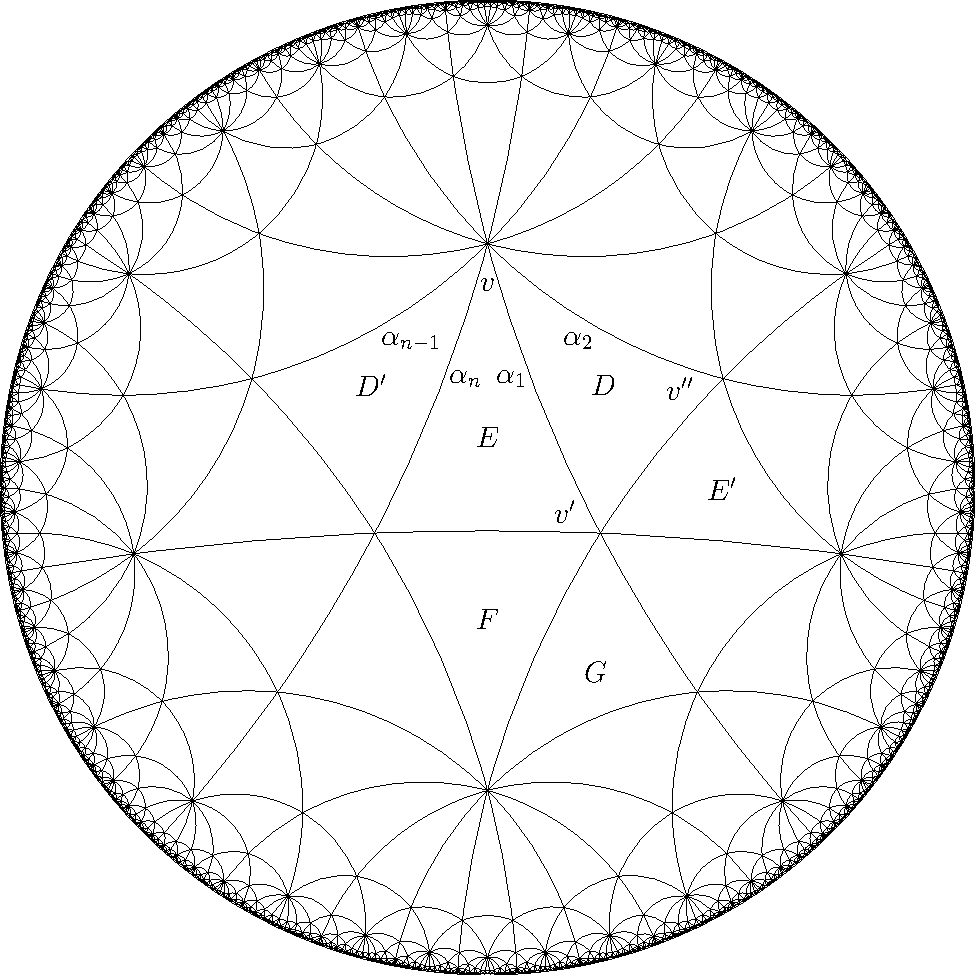
\includegraphics[width=4.5 in]{diagrams/deg33n.pdf}
\end{center}
\end{figure}


	Since $\partial\alpha_1$ separates $D$ and $E,$ we know that $D$ borders $\partial \alpha_2.$ We know that $D$ and $E'$ share two vertices, one of which is $v'.$ The other one cannot be $v$ as the only two chambers which share $v$ and $v'$ are $D,E$ and we assume $E'\neq E.$ Thus we can say that $D,E'$ share two vertices, $v,v''$ and $v''\neq v.$ As before, this means $|\st(v'')|=6.$ Since $D$ borders $\partial \alpha_2$ also know that two vertices of $D$ lie on $\partial \alpha_2.$ The vertex $v'$ cannot lie on $\partial\alpha_2$ as we know that $\partial\alpha_1$ contains $v$ and $v'$ and two distinct walls cannot share two vertices. Therfore, $v''$ lies on $\partial \alpha_2.$ 

	We have that $v''$ is a vertex of $\Sigma$ with $|\st(v'')|=6$ and thus $U_{v''}=U'_{v''}.$ We also know that $E'\in \st(v'')$ and $d(E',C)=d(D,C)-1=d(E,C)=k.$ Thus $d(\proj_{v''}(C),C)\le k.$ By Lemma \ref{lem:deg3fg} this means that $U_{v''}\subset U_k.$ But $\alpha_2$ is a positive root through $v''$ and thus $U_{\alpha_2}\subset U_k$ as desired.

	If $D'\in \st(v')$ from before, then identical arguments show that $U_{\alpha_{n-1}}\subset U_k$ which gives the desired result.
\end{proof}
It turn out that if $U_x$ is isomorphic to either $C_2(2)$ or $G_2(3)$ then the addition of $U_{\alpha_2}$ or $U_{\alpha_{n-1}}$ to $U_k$ will generated all of $U_v$ and we will use this to show that $U_+$ is finitely generated. We will state the result more precicely.
\begin{lemma}
\label{lem:exgen}	
Suppose $v$ is a vertex of $\Sigma$ and $\alpha_1,\dots,\alpha_n$ is a standard labeling of the positive roots through $v.$ If $U_v\cong C_2(2)$ or $G_2(3)$ then $U_v=\langle U_{\alpha_1},U_{\alpha_2},U_{\alpha_n}\rangle=\langle U_{\alpha_1},U_{\alpha_{n-1}},U_{\alpha_n}\rangle.$
\end{lemma}
\begin{proof}
	To prove the result, we will simply use the know presentations of $C_2(2)$ and $G_2(3)$ from the theory of Chevalley Groups. Let $H=\langle U_{\alpha_1},U_{\alpha_2},U_{\alpha_n}\rangle\le U_v$ and let $H'=\langle U_{\alpha_1},U_{\alpha_{n-1}},U_{\alpha_n}\rangle\le U_v.$ Also recall that $U_v$ is generated by $U_{\alpha_1},\dots,U_{\alpha_n}.$

	First suppose that $U_v\cong C_2(2),$ let $\alpha_1,\dots,\alpha_4$ be a standard labeling of the positive roots through $v,$ and let $U_i=U_{\alpha_i}$ for $1\le i \le 4.$ Then $U_i=\{1,u_i\}$ for all $i$ and we have the commutator relation $[u_1,u_4]=u_2u_3.$ Since $U_v$ is generated by $U_1,U_2,U_3,U_4,$ it will suffice to show that $U_3\subset H$ and $U_2\subset H'.$

	By definition, $U_1,U_2,U_4\subset H$ and thus $u_1,u_2,u_4\in H.$ This means $[u_1,u_4]\in H$ and thus $u_2[u_1,u_4]=u_2(u_2u_3)=u_3\in H$ so $U_3\subset H.$ This means $H=U_v$ which gives the desired result. A similar argument shows that $[u_1,u_4]u_3=u_2\in H'$ and thus $U_2\in H'.$ Thus $H'=U_v$ as desired.

	Now suppose that $U_v$ cong $G_2(3).$ Then $U_{\alpha_i}$ is a cyclic group of orderer 3 for every positive root $\alpha_i$ through $v.$ Recall that for any group $G,$ we will let $G^*$ denote the non-trivial elements of $G.$ There is a standard labeling $\alpha_1,\dots,\alpha_6$ of the positive roots through $v$ so that we get the following commutator relations
	\begin{align*}
		[U^*_1,U^*_6]&\subset U^*_2U^*_3U^*_4U^*_5\\
		[U^*_2,U^*_6]&=U^*_4\\
		[U^*_1,U^*_5]&=U^*_3\\
		[U^*_i,U^*_j]&=\{1\} \text{ for all other }i,j
	\end{align*}
	where $U_i=U_{\alpha_i}.$ 

	Now let $H$ be a subgroup of $U_v$ which contains $U_1,U_2,U_6.$ Then we know that $U'_v\le H\le U_v$ and $[U_v:U'_v]=3$ so either $H=U'_v$ or $H=U_v.$ A fact from group theory states that $\langle A,B\rangle=A[A,B]B$ and thus we have $U'_v=U_1U^*_2U^*_3U^*_4U^*_5U_6\cup\{1\}.$ This means $U_2$ is not contained in $U'_v$ as non-trivial elements of $U_2$ cannot be written in this form. Since $U_2\subset H$ and $U_2\not\subset U'_v$ we can conclude that $H=U_v$ so $U_v$ is generated by $U_1,U_2,$ and $U_6$ as desired. An identical argument shows that $U_v$ is also generated by $U_1,U_5,U_6$ which gives the result.

	\textcolor{red}{Peter: I probably should move this proof to background. I also don't know if this is the best way to prove this result so maybe we can discuss this soon.}
\end{proof}

Before we proceed with the main proof, there is one more idea about roots we need to define. If $D$ is a chamber of $\Sigma$ and $\alpha$ is a root of $\Sigma,$ then we will say that $D$ \emph{borders} $\alpha$ if a panel of $D$ lies on $\partial\alpha.$  If $\alpha$ is a positive root of $\Sigma$ then we can define $d(\alpha,C)$ to be the minimum of $d(D,C)$ where $D$ is a chamber which borders $\alpha.$ If $d(\alpha,C)=n$ then there is a chamber $D$ bordering $\alpha$ such that $d(\alpha,C)=d(D,C)$ and $D$ must be contained in $\alpha.$ 

We are now ready to proceed with the main result of this section.

\begin{theorem}
	\label{thm:334fg}
	Let $(G,(U_\alpha)_{\alpha\in \Phi},T)$ is an RGD system of type $(W,S)$ such that $S=\{s,t,u\}$ and $m(s,t)=m(s,u)=3$ and $m(t,u)=4$ or $6.$ If $x$ is the vertex of the fundamental chamber $C$ of type $s,$ and $U_x\cong C_2(2)$ or $U_x\cong G_2(3)$ then $U_+$ is finitely generated.
\end{theorem}
\begin{proof}
	For each $k\ge 1$ let $U_k=\langle U_\alpha|d(\alpha,C)\le k\rangle\le U_+.$ We can immediately deduce the following facts. We know that $U_1\subset U_2\subset \cdots$  and $\cup_{k\ge 1} U_k=U_+$ since every root will be some finite distance from $C.$ For any $k,$ there are only finitely many chamber of $\Sigma$ distance less that $k$ away from $C,$ and each chamber will border 3 distinct roots. Thus there are only finitely many roots $\alpha$ with $d(\alpha,C)\le k$ and so $U_k$ is finitely generated for all $k.$ We will show that $U_k\subset U_{k-1}$ for $k\ge 3$ which will show that $U_+$ is finitely generated.

	Let $k\ge 3$ and choose $\gamma\in \Phi_+$ such that $d(\gamma,C)=k.$ Then we can find a chamber $D$ of $\Sigma$ which borders $\gamma$ such that $d(\gamma,C)=d(D,C)=k.$ Let $D'$ be a chamber adjacent $D$ which is closer to $C,$ or in other words, $d(D',C)=d(D,C)-1.$ Since $D$ borders $\gamma$ we know that $D$ will have two vertices on $\partial \gamma,$ and we also know that $D$ and $D'$ will share two vertiex, which means one of the common vertices will also lie on $\partial\gamma.$ Let $v$ be a vertex shared by $D$ and $D'$ which lies on $\partial \gamma.$ By definition, this means $\gamma$ is a positive root at $v$ and thus $U_\gamma\subset U_v.$

	Let $E=\proj_v(C).$ Then $E$ is the chamber in $\st(v)$ which minimizes the distance to $C.$ Since $D'\in \st(v)$ and $d(D',C)<d(D,C)$ we know that $E\neq D$ and $l=d(E,C)<d(D,C)=k.$ There are exactly two possibilites for $v.$ If $v$ is a vertex of type $t$ or $u$ then $|\st(v)|=6$ and $U_v=U'_v.$ Then we can apply Lemma \ref{lem:deg3fg} to see that $U_v\subset U_l\subset U_{k-1},$ and since $U_\gamma \subset U_v$ we know that $U_\gamma \subset U_{k-1}$ as desired.

	Now suppose that $v$ is a vertex of type $s.$ Then by Lemma \ref{cor:respectphiv} we know that $U_v\cong U_x\cong C_2(2)$ or $G_2(3).$ Let $\alpha_1,\dots,\alpha_n$ be a standard labeling of the positive roots through $v.$ Once again we have two possibilities. If $d(E,C)=l\ge 2$ then we can apply Lemma \ref{lem:exdegfg} to see that at least one of $U_{\alpha_2}$ or $U_{\alpha_{n-1}}$ is contained in $U_l\subset U_{k-1}.$ If $d(E,C)<2$ then we have $U_{\alpha_2},U_{\alpha_{n-1}}\subset U_2\subset U_{k-1}$ by definition and by choice of $k.$ In either case we have shown that at least on of $U_{\alpha_2}$ and $U_{\alpha_{n-1}}$ is contained in $U_{k-1}.$ By Lemma \ref{lem:exgen} this means that $U_v\subset U_{k-1}$ and thus $U_\gamma\subset U_{k-1}.$

	Since the choice of $\gamma$ was arbitrary we have shown that $U_\gamma \subset U_{k-1}$ for all positive roots $\gamma$ such that $d(\gamma,C)=k\ge 3.$ Thus we have $U_k\subset U_{k-1}$ for all $k\ge 3,$ and inducitvely this shows that $U_k=U_2$ for all $k\ge 3.$ But this means $U_+=U_2$ and so $U_+$ is finitely generated by all positive root groups of distance at most two away from $C$ as desired.

\end{proof}

\end{document}
